\documentclass[twoside,11pt]{article}

\usepackage{aa228-jmlr2e}
\usepackage{lipsum}
\usepackage{listings}

\input{julia_listing}

\begin{document}

% Refer to this link for project rubric: https://aa228.stanford.edu/project-1/
\title{Project 1: Bayesian Structure Learning}

%===========================================
% TODO: Replace "First Last" with your name.
% TODO: Replace "email@stanford.edu" with your Stanford email.
%===========================================
\name{Brandon DAgostino}
\email{bdag@stanford.edu}


\maketitle


\section{Algorithm Description}
%===========================================
% TODO: Replace this with a short description of your algorithm(s) used.
The structure learning approach implemented in this project is a simple directed graph search using the K2 algorithm and
Bayesian score. The approach follows closely with the reference implementation presented in Algorithm 5.2 in book
section 5.2 and proceeds as follows:

\begin{enumerate}
  \item A new unconnected graph is initialized with nodes corresponding to each variable in the dataset. The Bayesian
    score is computed for the empty graph, which is the initial best score.
  \item For each node in a provided node ordering, the algorithm iteratively considers adding a directed edge from each
    preceding node in the ordering to the current node. If adding the edge improves the Bayesian score, the edge is
    added to the graph and the best score is updated. This process continues until no more edges can be added that
    improve the score or a maximum number of parents is reached.

    Both the node ordering and maximum number of parents are provided as input parameters to the algorithm, and default
    to the natural ordering of the variables and infinity (i.e., no limit), respectively.
  \item The final graph structure and resulting Bayesian score is returned after all nodes have been processed.
\end{enumerate}

The full Julia implementation is presented along with its supporting code in Section~\ref{sec:code}. The program runtime
(excluding compilation time) and figure reference for the resulting Bayesian network of each dataset is presented below
in Table~\ref{tab:runtimes}.

\begin{table}[h!]
  \centering
  \begin{tabular}{|c|c|c|}
    \hline
    Dataset & Runtime (s) & Figure \\
    \hline
    Small & 0.229 & 1 \\
    Medium & 8.899 & 2 \\
    Large & 1363.306 & 3 \\
    \hline
  \end{tabular}
  \caption{Program runtimes and figure references for each dataset.}
  \label{tab:runtimes}
\end{table}

%===========================================


\newpage
\section{Graphs}
%===========================================
% TODO: Add your small, medium, and large graph visualizations here
%===========================================
\begin{figure}[h!]\label{graph:small}
  \centering
  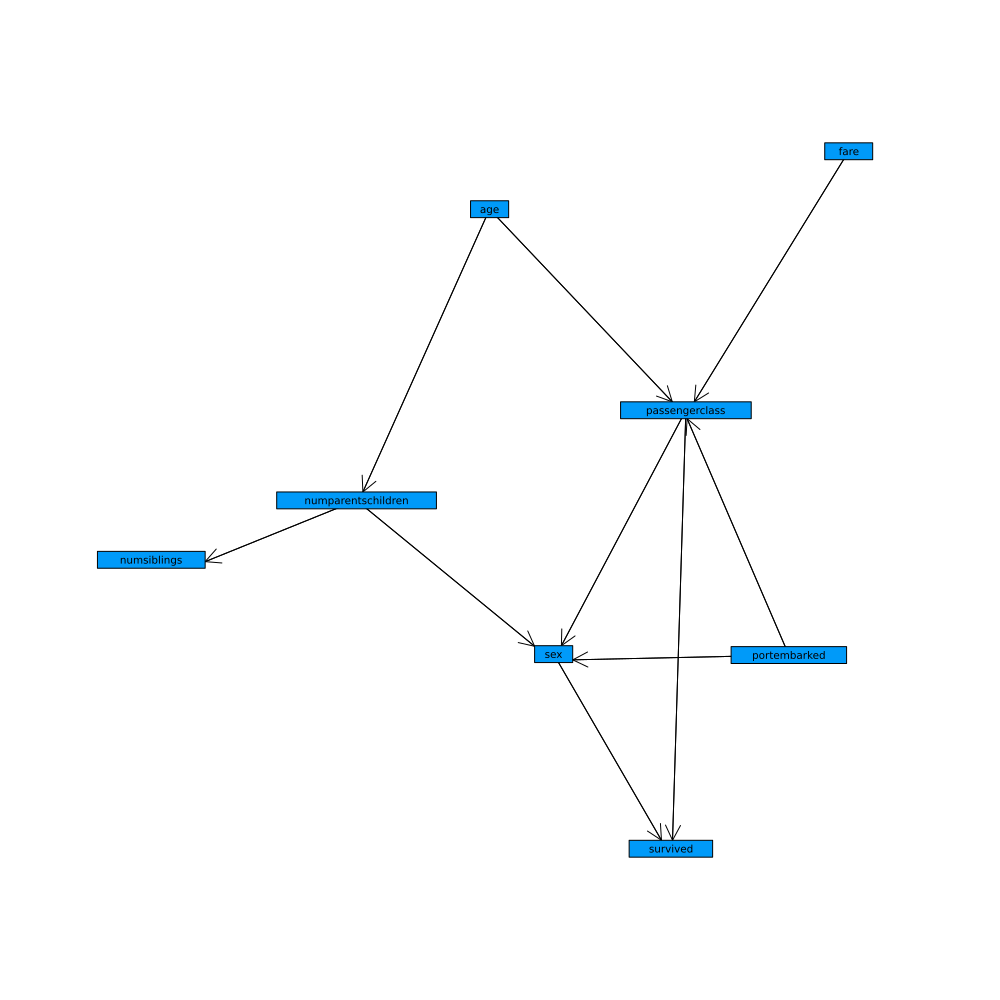
\includegraphics[width=0.5\textwidth]{../output/small.png}
  \caption{Bayesian Network for small dataset.}
\end{figure}

\begin{figure}[h!]\label{graph:med}
  \centering
  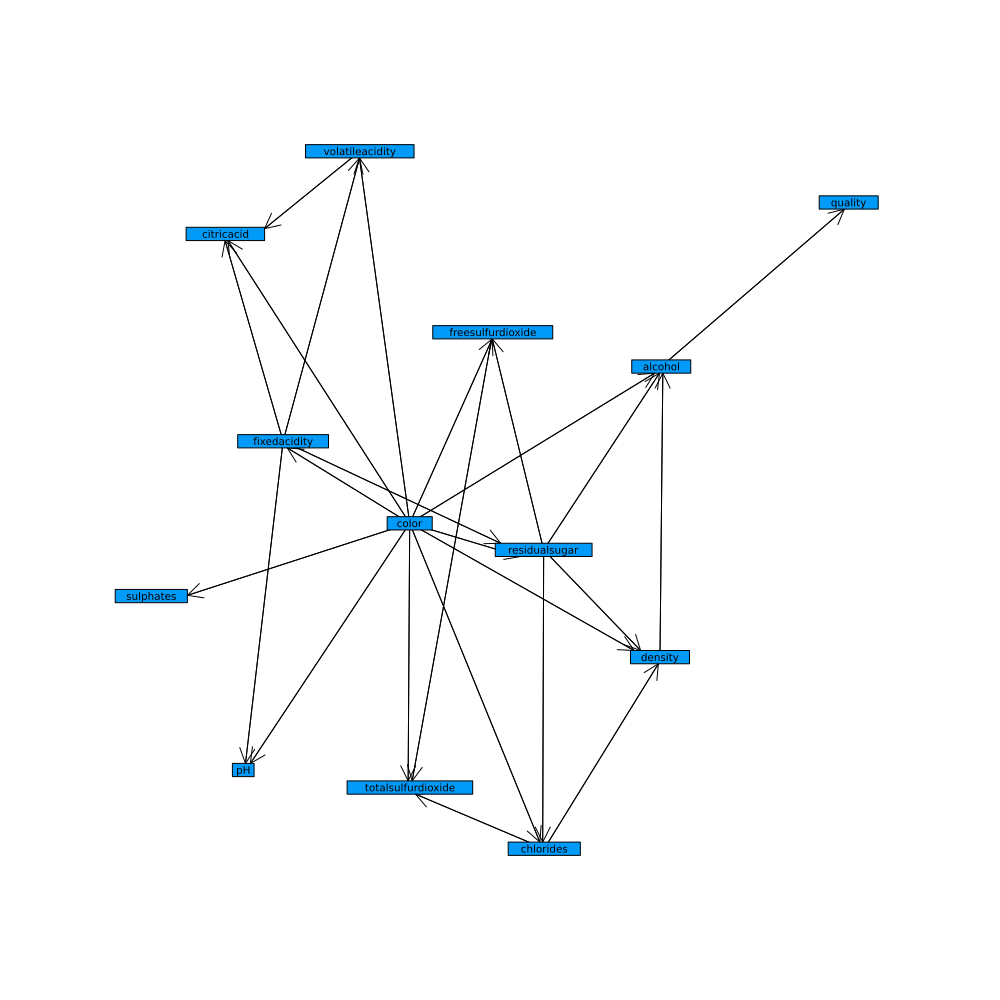
\includegraphics[width=0.5\textwidth]{../output/medium.png}
  \caption{Bayesian Network for medium dataset.}
\end{figure}

\begin{figure}[h!]\label{graph:large}
  \centering
  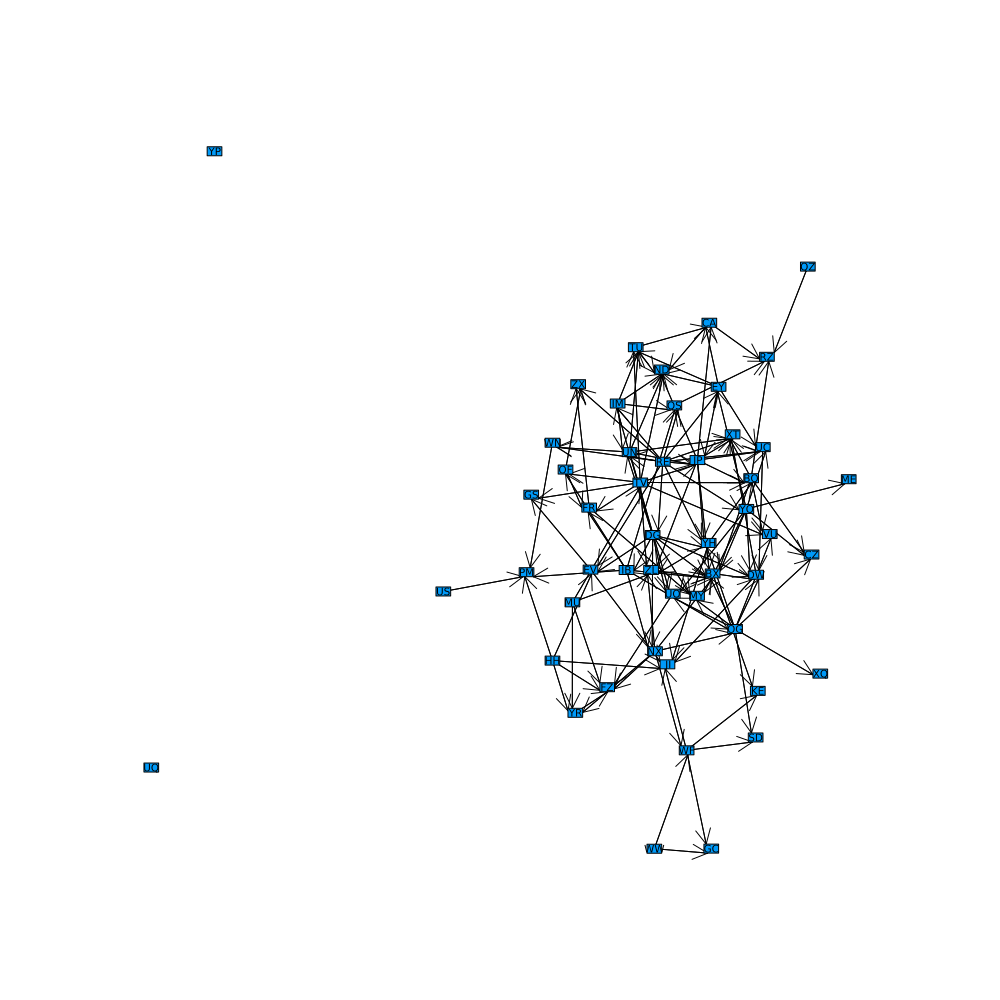
\includegraphics[width=0.5\textwidth]{../output/large.png}
  \caption{Bayesian Network for large dataset.}
\end{figure}


\newpage
\section{Code}\label{sec:code}
%===========================================
% TODO: Add your code here, see code listing options here: https://www.overleaf.com/learn/latex/code_listing
% NOTE: Code does not count towards your page limit!
% OPTIONS:
%   1. Paste everything into a {verbatim} environment (where all characters are parsed...verbatim).
%   or 2. paste everything into a {lstlisting} environment for syntax highlighting (examples for Julia and Python below).
% NOTE: Feel free to break up functions into separate {algorithm} + {lstlisting} environments for better organization (not required!)
%===========================================


%===========================================
% EXAMPLE JULIA: TODO REPLACE WITH YOUR CODE
%===========================================
\begin{algorithm}
  \lstinputlisting[language=Julia]{../project1.jl}
\end{algorithm}


\end{document}
